\documentclass{beamer}
\usepackage{bookmark}
\usepackage{beamerthemeBerkeley}
\usepackage{color}
\usepackage{amsmath}
\usepackage{hyperref}
\hypersetup{colorlinks,linkcolor=blue,citecolor=blue}
\usepackage{listings}
\usepackage{xcolor}
\usepackage{graphicx}
\usepackage{amsfonts}
\usecolortheme{default}
\usetheme{Berkeley}

\definecolor{dkgreen}{rgb}{0,0.6,0}
\definecolor{gray}{rgb}{0.5,0.5,0.5}
\definecolor{mauve}{rgb}{0.58,0,0.82}

\lstset{
  basicstyle=\footnotesize, 
  numbers=left, 
  numberstyle=\tiny\color{gray}, 
  stepnumber=1,
  numbersep=5pt, 
  backgroundcolor=\color{white},
  showspaces=false,
  showstringspaces=false,
  showtabs=false,
  frame=trbl,
  rulecolor=\color{black},
  tabsize=2,
  captionpos=b,
  breaklines=true, 
  breakatwhitespace=false, 
  title=\lstname,
  keywordstyle=\color{blue},
  commentstyle=\color{dkgreen},
  escapeinside={\%*}{*)}, 
  morekeywords={*,...} 
}
\title{Lab Presentation \\Kernel Arguments (Linux)}
\author{VE482 Team 1}
\institute{UM-SJTU Joint Institute}
\date{\today}

\begin{document}
\begin{frame}
	\titlepage
\end{frame}

\begin{frame}
	\tableofcontents
\end{frame}

\begin{frame}
	\section{Introduction}
	\frametitle{What are kernel arguments?}
	
	\begin{block}{Definition}
		{\color{blue} kernel arguments}, also known as Kernel parameters, are used to customize the behavior of OS.
	\end{block}
	
	There are three ways to pass options to the kernel and thus control its behaviour:
	\begin{itemize}
	    \item When building the kernel. 
\item When starting the kernel (usually, when invoked from a boot loader).
\item At runtime (through the files in /proc and /sys). 
	\end{itemize}
\end{frame}

\begin{frame}
\frametitle{Kernel arguments list}
\begin{figure}[H]
    \centering
    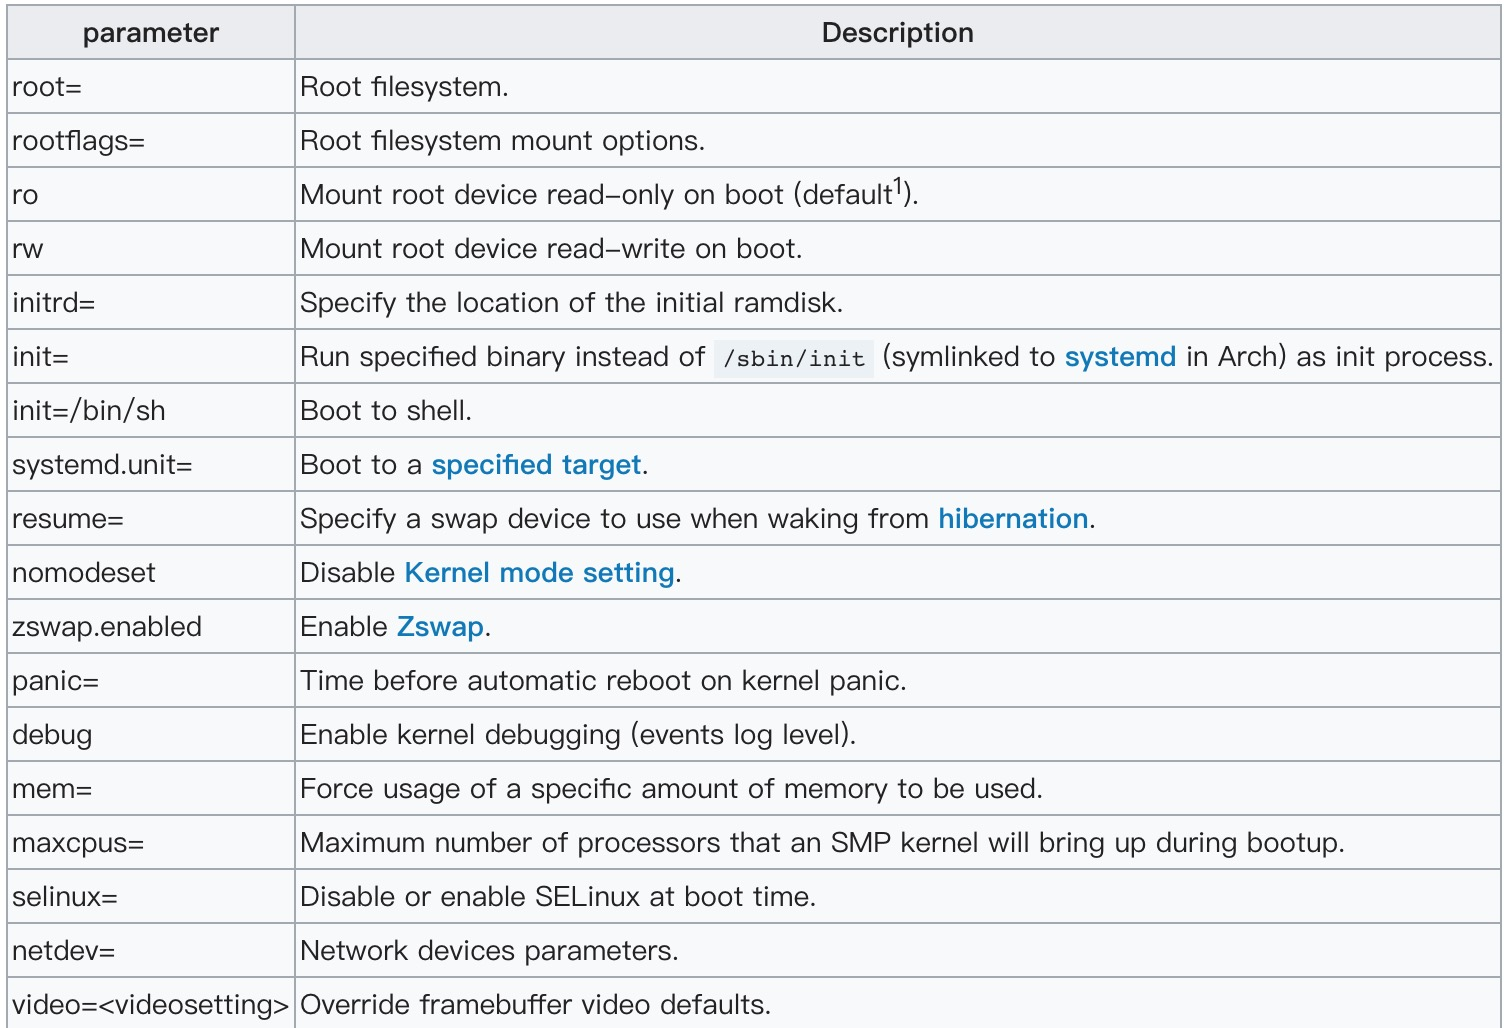
\includegraphics[width=\textwidth]{1.jpg}
\end{figure}
    
\end{frame}

\begin{frame}{Notes}
    \begin{itemize}
        \item Not all parameters are always available. Most are associated with subsystems and work only if the kernel is configured with those subsystems built in. They also depend on the presence of the hardware they are associated with.
\\
\item Parameters either have the format parameter or parameter=value.
\\
 \item All kernel parameters are case-sensitive. Most of them are lower case, writing those in upper case does not work.
    \end{itemize}

\end{frame}

\begin{frame}
    \section{Configuration}
    \subsection{Building}
    \frametitle{Configure on Building}
    The first way is to set the parameters before compilation. Kernel configuration is set in its {\color{blue} .config} file and properly set it can change the configuration.

    \begin{block}{More Advanced Configuration}
        \begin{itemize}
            \item menuconfig, nconfig - menulized configuraiton
            \item xconfig, gconfig - GUI configuration which requires graphical support
        \end{itemize}
    \end{block}

\end{frame}

\begin{frame}[fragile]
	\subsection{Booting}
	\frametitle{On Booting}
	\begin{block}{GRUB}
	 \begin{itemize}
       \item Press 'e' when the menu shows up and add them on the linux line:
       \begin{lstlisting}
linux /boot/vmlinuz-linux root=UUID=978e3e81-8048-4ae1-8a06-aa727458e8ff quiet splash
       \end{lstlisting}
       Press Ctrl+x to boot with these parameters.
     \end{itemize}
	\end{block}
	
\end{frame}



\begin{frame}[fragile]
	\begin{block}{GRUB}
	 \begin{itemize}
       \item To make the change persistent after reboot, while you could manually edit /boot/grub/grub.cfg with the exact line from above, the best practice is to:\\
\vspace{0.5cm}
Edit /etc/default/grub and append your kernel options to the GRUB$\_$CMDLINE$\_$LINUX$\_$DEFAULT line:
\begin{lstlisting}
GRUB_CMDLINE_LINUX_DEFAULT="quiet splash"
\end{lstlisting}
And then automatically re-generate the grub.cfg file with:
\begin{lstlisting}
# grub-mkconfig -o /boot/grub/grub.cfg
\end{lstlisting}
     \end{itemize}
	\end{block}
	
\end{frame}

\begin{frame}[fragile]
    \subsection{Runtime}
	\frametitle{In Runtime}
	Some kernel arguments can also be modified in runtime, and there are mainly two ways to do this.
	\begin{block}{Using procfs}
		Kernel arguments are saved as files in the proc file systems (which is always mounted at /proc in linux) directly write to the files can change the kernel arguments.
	\end{block}
    The basic step is using {\color{blue} echo} to change these files.

    
    \begin{lstlisting}[language=bash]
    echo SOME_VALUE > /proc/sys/SOME_DIRECTORY/SOME_FILE
    \end{lstlisting}
    
\end{frame}

\begin{frame}
    \begin{block}{Using sysctl}
        {\color{blue}sysctl }is a command to configure kernel parameters. There are two ways to use it
        \begin{itemize}
            \item sysctl SOME\_PARAMETER=SOME\_VALUE
            \item Edit the configuration file (/etc/sysctl.conf) and run "sysctl -p"
        \end{itemize}
    \end{block}
	
\end{frame}


\begin{frame}
	\section{References}
	\frametitle{References}
	\begin{itemize}
		\item \url{https://wiki.archlinux.org/index.php/Sysctl}
		\item \url{https://www.ibm.com/developerworks/library/l-proc/index.html}
		\item \url{https://wiki.archlinux.org/index.php/Kernel_parameters}
	\end{itemize}
\end{frame}

\end{document}